\section{Performance Evaluation, Results, Discussion}

\textit{owners: Evan: graphs, All: interpretation (2.75 pages)}

\begin{itemize}
\item Platform Descriptions
\begin{itemize}
  \item EC2

  \item XC40
  \item Experimental Cray Cluster (EXP\_CC)
\end{itemize}

\item CX Spark Implementation Phase Descriptions
 \begin{enumerate}
      \item Load Matrix Metadata
      \item Load Matrix
      \item Iterations
      \item Postprocessing/Collect
 \end{enumerate}

 \item Dataset Sizes
 \begin{itemize}
  \item 100GB

  \item 1 TB

\end{itemize}
 \end{itemize}




  \subsection{Single Node Scaling Table}

  \begin{center}
  \begin{tabular}{ |c|c|c| } 
  \hline
  Single Node Optimization & Overall Speedup\\
  \hline
  Original Implementation & 1.0  \\
  Multi-Core Synchronization & 6.5 \\
  Cache Blocking & 15.6 \\
  SIMD & 39.7 \\
  \hline

  \end{tabular}
  \end{center}
  \textbf{Table 1: Single node optimizations to the CX C implementation and the subsequent speedup each additional optimization provides}

  In Table~\ref{tab:fdsfds}, we show the benefits of various
  optimizations described in Sec.~\ref{sec:fdsd} on a single-node of our Spark system. 
  The matrix $\mathcal{A}$ has {\it{m}} = 1.95M, {\it{n}} = 128K,
  {\it{s}} = 0.004, and {\it{nnz}} = 10$^9$. The rank parameter,
  {\it{k}} = 32. We started with a parallelized implementation,
  without any of the described optimizations, and measured the 
  performance (in terms of time taken). We first implemented the 
  multi-core synchronization scheme, wherein a single copy of the 
  output matrix is kept (for the matrix multiplication).
  This resulted in a speedup of around 6.5X, primarily due to
  the reduction in the amount of data traffic between the 
  last-level cache and main memory (there was around 19X measured reduction
  in traffic). We then implemented our cache blocking scheme,
  primarily targetted towards ensuring that the output of the 
  matrix multiplication resides in the caches (since it is
  accessed and updated frequently). This led to a further 2.4X
 reduction in run-time, for an overall speedup of around 15.6X.

 Once the memory traffic was optimized for, we implemented our 
 SIMD code, by vectorizing the element-row multiplication-add
 operations (described in detail in Sec.~\ref{sec:fdsfdsfds}). 
 The resultant code sped up by a further 2.6X, for an overall
 speedup of 39.7X. Although the effective SIMD width
 ($\mathcal{S}$ = 4), there are overheads of address computation,
 stores, and not all computations were vectorized (QR code is still
 scalar).
 



  \subsection{Scaling}
    \begin{figure} [H]
    \begin{centering}
    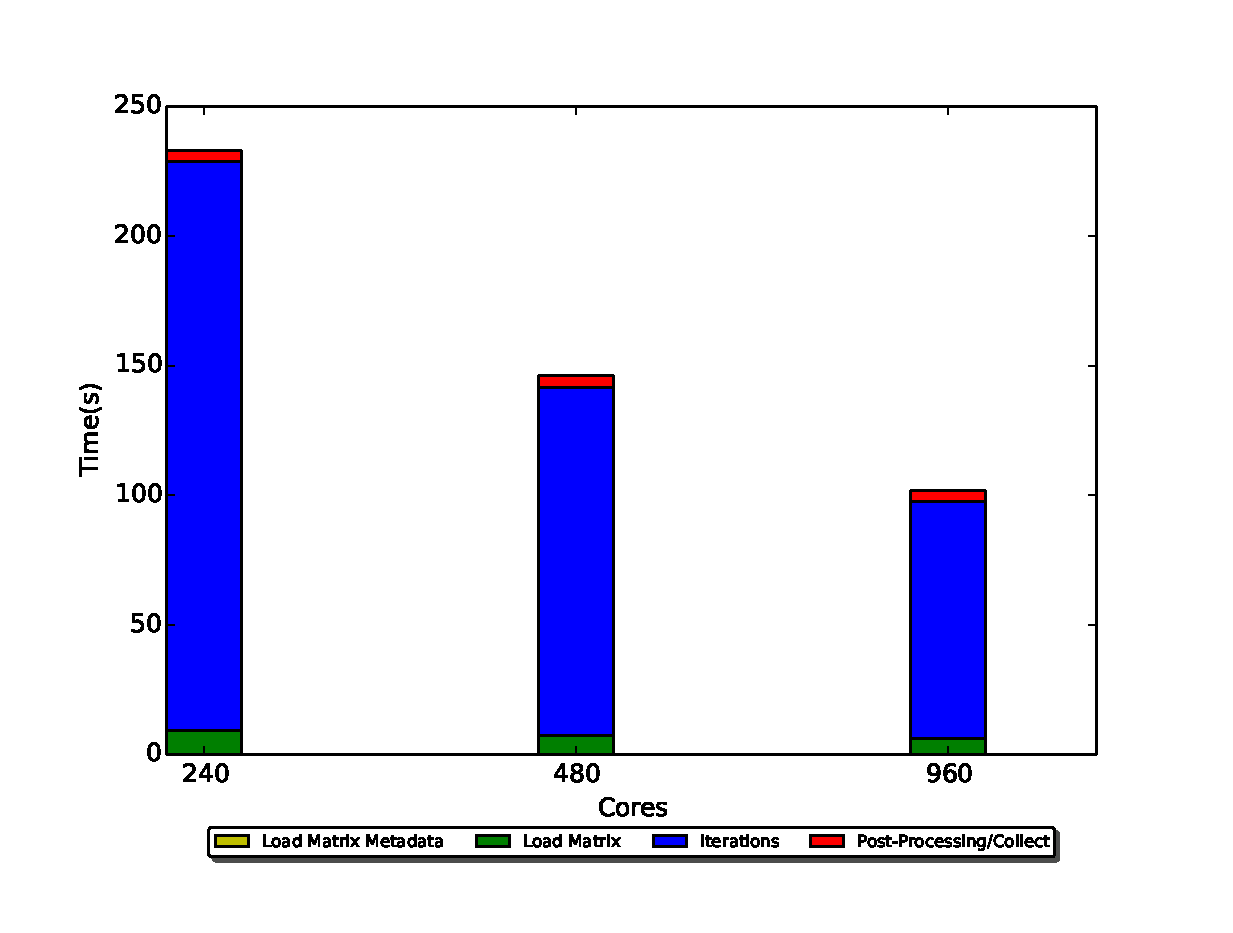
\includegraphics[scale=0.4]{images/CX_Strong_Scaling_Rank_32_Partitions_default.eps}
    \end{centering}
    \caption{ Strong scaling for the 4 phases of CX on an XC40 for 100GB dataset at rank 32 and default partitioning as concurrency is increased.} 
    \end{figure} 


  \subsection{Dataset Size Scaling Across Platforms}
    
    \begin{figure} [H]
    \begin{centering}
    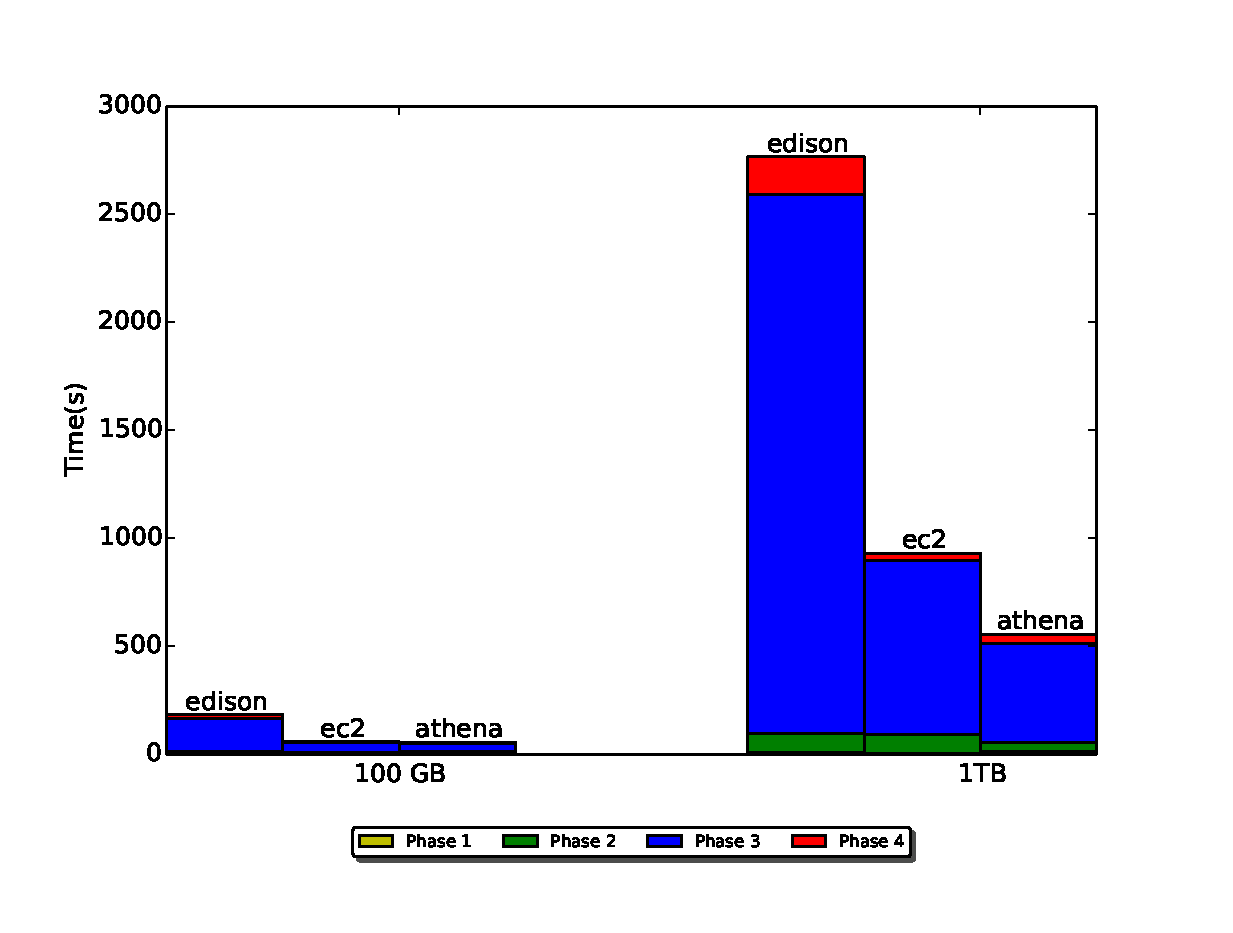
\includegraphics[scale=0.4]{images/CX_Size_Scaling_Rank_16_Partitions_default.eps}
    \end{centering}
    \caption{ Run times for the various stages of computation for CX for two different dataset sizes for the three platforms using rank 16 and default partitioning for the given platform} 
    \end{figure}

      \begin{figure} [H]
    \begin{centering}
    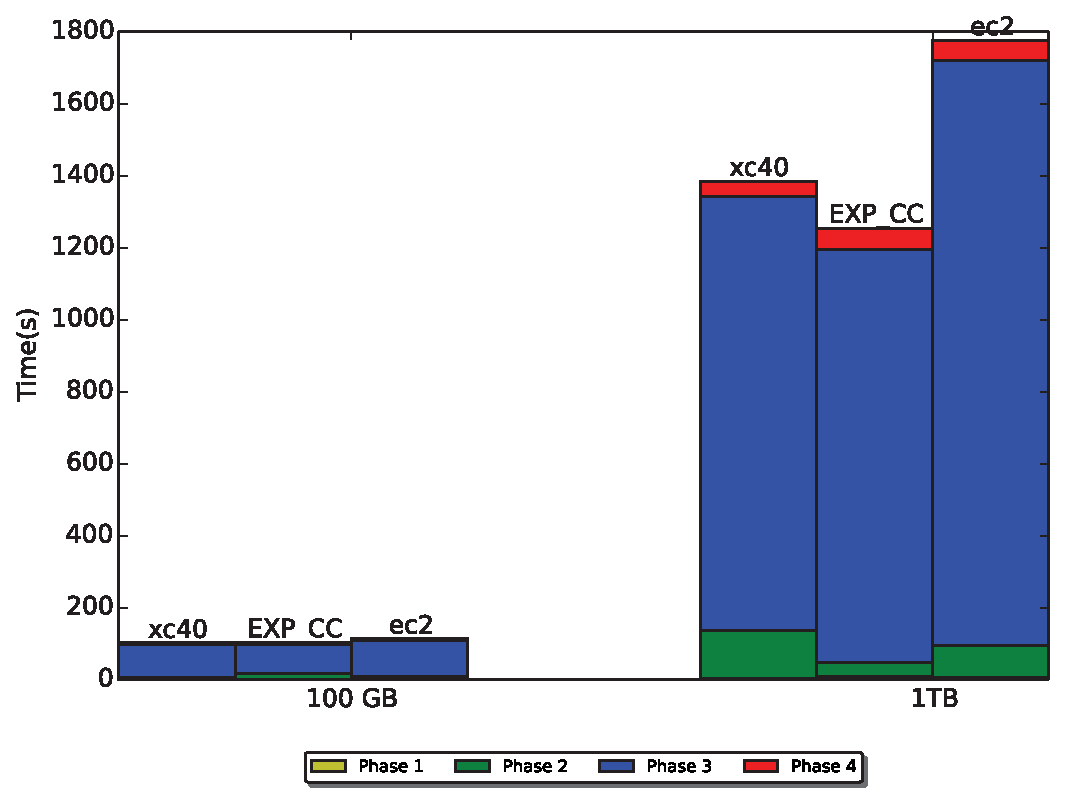
\includegraphics[scale=0.4]{images/CX_Size_Scaling_Rank_32_Partitions_default.eps}
    \end{centering}
    \caption{ Run times for the various stages of computation for CX for two different dataset sizes for the three platforms using rank 32 and default partitioning for the given platform} 
    \end{figure}
  

  \subsection{Comparison of CX, PCA, RPCA quantitatively (Alex will work on this)? }
    \begin{itemize}
      \item (for 100GB sized dataset on EC2)
      \item runtime vs. accuracy?
      \item show distinction b/w cx, pca
      \item alex will take ownership
    \end{itemize}

  \subsection{Science plot for PCA, CX (Jiyan and Oliver will produce this)}

